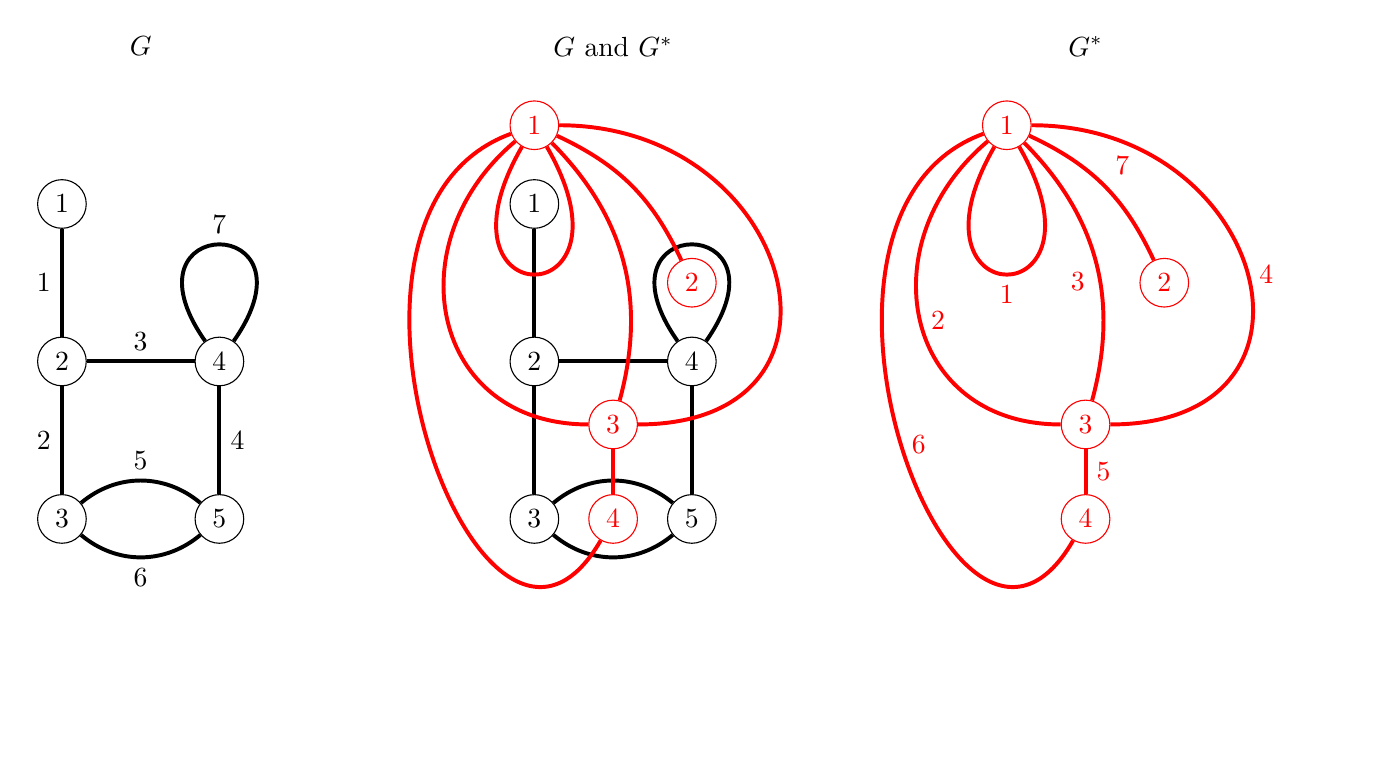
\begin{tikzpicture}
	\begin{scope}[xshift=0cm, yshift=0cm]
		\node (G) at (1, 6) {$G$};

		\node[circle, draw] (a1) at (0, 4) {1};
		\node[circle, draw] (a2) at (0, 2) {2};
		\node[circle, draw] (a3) at (0, 0) {3};
		\node[circle, draw] (a4) at (2, 2) {4};
		\node[circle, draw] (a5) at (2, 0) {5};
	
		% Draw the edges between nodes with labels
		\draw[line width=0.5mm] (a1) -- node[left] {1} (a2);
		\draw[line width=0.5mm] (a2) -- node[left] {2} (a3);
		\draw[line width=0.5mm] (a2) -- node[above] {3} (a4);
		\draw[line width=0.5mm] (a4) -- node[right] {4} (a5);
		\draw[line width=0.5mm] (a3) to[bend left=40] node[above] {5} (a5);
		\draw[line width=0.5mm] (a3) to[bend right=40] node[below] {6} (a5);
		\draw[line width=0.5mm] (a4) to[in=125,out=55,loop, min distance=2cm] node[above] {7} (a4);
	\end{scope}

	\begin{scope}[xshift=6cm, yshift=0cm]
		\node (G) at (1, 6) {$G$ and $G^*$};

		\node[circle, draw] (a1) at (0, 4) {1};
		\node[circle, draw] (a2) at (0, 2) {2};
		\node[circle, draw] (a3) at (0, 0) {3};
		\node[circle, draw] (a4) at (2, 2) {4};
		\node[circle, draw] (a5) at (2, 0) {5};
	
		% Draw the edges between nodes with labels
		\draw[line width=0.5mm] (a1) -- (a2);
		\draw[line width=0.5mm] (a2) -- (a3);
		\draw[line width=0.5mm] (a2) -- (a4);
		\draw[line width=0.5mm] (a4) -- (a5);
		\draw[line width=0.5mm] (a3) to[bend left=40] (a5);
		\draw[line width=0.5mm] (a3) to[bend right=40] (a5);
		\draw[line width=0.5mm] (a4) to[in=125,out=55,loop, min distance=2cm] (a4);

		\node[circle, draw, color=red, fill=white] (d1) at (0, 5) {1};
		\node[circle, draw, color=red, fill=white] (d2) at (2, 3) {2};
		\node[circle, draw, color=red, fill=white] (d3) at (1, 1.2) {3};
		\node[circle, draw, color=red, fill=white] (d4) at (1, 0) {4};
		
		\draw[line width=0.5mm, color=red] (d1) to[in=240, out=300, loop, min distance=2.5cm] (d1);
		\draw[line width=0.5mm, color=red] (d1) to[bend left=20] (d2);
		\draw[line width=0.5mm, color=red] (d1) to[bend left=30] (d3);
		\draw[line width=0.5mm, color=red] (d1) to[in=180, out=220, min distance=2cm] (d3);
		\draw[line width=0.5mm, color=red] (d1) to[in=0, out=0, min distance=3cm] (d3);
		\draw[line width=0.5mm, color=red] (d3) -- (d4);
		\draw[line width=0.5mm, color=red] (d1) to[in=240, out=200, min distance=3cm] (d4);
	\end{scope}

	\begin{scope}[xshift=12cm, yshift=0cm]
		\node (G) at (1, 6) {$G^*$};

		\node[circle, draw, color=red, fill=white] (d1) at (0, 5) {1};
		\node[circle, draw, color=red, fill=white] (d2) at (2, 3) {2};
		\node[circle, draw, color=red, fill=white] (d3) at (1, 1.2) {3};
		\node[circle, draw, color=red, fill=white] (d4) at (1, 0) {4};
		
		\draw[line width=0.5mm, color=red] (d1) to[in=240, out=300, loop, min distance=2.5cm] node[below] {1} (d1);
		\draw[line width=0.5mm, color=red] (d1) to[in=180, out=220, min distance=2cm] node[right] {2} (d3);
		\draw[line width=0.5mm, color=red] (d1) to[bend left=30] node[below left] {3} (d3);
		\draw[line width=0.5mm, color=red] (d1) to[in=0, out=0, min distance=3cm] node[right] {4} (d3);
		\draw[line width=0.5mm, color=red] (d3) to node[right] {5} (d4);
		\draw[line width=0.5mm, color=red] (d1) to[in=240, out=200, min distance=3cm] node[right] {6} (d4);
		\draw[line width=0.5mm, color=red] (d1) to[bend left=20] node[above right] {7} (d2);
	\end{scope}
\end{tikzpicture}
